\documentclass{article}
\usepackage{listings}
\usepackage{xcolor}
\usepackage{aligned-overset}
\usepackage{bookmark}
\usepackage{fancyhdr}
\usepackage{array}
\usepackage{appendix}
\usepackage{bm}
\usepackage{chapterbib}
\usepackage{float}
\usepackage[UTF8]{ctex}
\usepackage{geometry}
\usepackage{natbib}
\usepackage{url}
\usepackage{graphicx}
\renewcommand\arraystretch{2}
\usepackage{subfigure}
\usepackage{enumerate}
\geometry{left=2.18cm,right=2.08cm,top=1.84cm,bottom=1.84cm}
\usepackage{graphicx}
\pagestyle{plain}	
\usepackage{setspace}
\usepackage{indentfirst}
\usepackage{caption2}
\usepackage{datetime} %日期
\renewcommand{\today}{\number\year 年 \number\month 月 \number\day 日}
\renewcommand{\captionlabelfont}{\small}
\renewcommand{\captionfont}{\small}
\usepackage{pythonhighlight}
\setlength{\parindent}{2em}
\lstset{language=Matlab}%代码语言使用的是matlab

\lstset{breaklines}%自动将长的代码行换行排版
\lstset{
    language    = c++,
    numbers     = left,
    numberstyle = \small,
    breaklines  = true,
    captionpos  = b,
    tabsize     = 4,
%   frame       = shadowbox,
    frame       = leftline,
    columns     = fullflexible,
    commentstyle = \commentFont\color[RGB]{0,0,0},
    keywordstyle = \codeBold\color[RGB]{0,0,0},
    basicstyle   = \small\codeFont,
    stringstyle  = \color[RGB]{48,0,20}\codeFont,
    rulesepcolor = \color{red!20!green!20!blue!20},
    showstringspaces = false,
}
\lstset{extendedchars=false}%解决代码跨页时,章节标题,页眉等汉字不显示的问题
\title{基于SIR模型对武汉新型冠状病毒疫情分析} 
\date{} 
\begin{document}
\begin{figure}
    \centering
    
\includegraphics[width=8cm]{upc.png}

    \label{figupc}
\end{figure}

  \begin{center}
    \quad \\
    \quad \\
    \heiti \fontsize{45}{17} \quad \quad \quad 
    \vskip 1.5cm
    \heiti \zihao{2} 数字图像处理实验
  \end{center}
  \vskip 2.0cm
    
  \begin{quotation}
%   \begin{center}
    \doublespacing
    
        \zihao{4}\par\setlength\parindent{7em}
    \qquad 

    学生姓名:\underline{\qquad  张世琛 \qquad \qquad}

    学\hspace{0.61cm} 号:\underline{\qquad 1804030401\qquad}
    
    专业班级:\underline{\qquad 计科1802 \qquad  }
    
    学\hspace{0.61cm} 院:\underline{计算机科学与技术学院}
%   \end{center}
    \vskip 5cm
    \centering
    % \begin{table}[h]
    %         \centering 
    %         \zihao{4}
    %         \begin{tabular}{|c|c|c|c|c|c|c|}
    %         % 这里的rl 与表格对应可以看到,姓名是r,右对齐的;学号是l,左对齐的;若想居中,使用c关键字。
    %             \hline
    %             课程认识 & 问题思 考 & 格式规范  & IT工具  & Latex附加  & 总分 & 评阅教师 \\
    %             30\% & 30\% & 20\% & 20\% & 10\% &  &  \\
    %             \hline
    %              & & & & & &\\
    %             & & & & & &\\
    %             \hline
    %         \end{tabular}
    %     \end{table}
    \vskip 2cm
    \today
  \end{quotation}

\thispagestyle{empty}
\newpage

\setcounter{page}{1}
%\maketitle
\section{直方图均衡化}
\subsection{代码编写的简单思路}
\subsubsection{挑选一张合适的原始图像}

  如图
                \begin{figure}[h!]
                \centering
                
\includegraphics[width=5.5cm,height=8cm]{xuan.png}
                \caption{原始图像}
                \end{figure}

  \subsubsection{先读入原始图像,转化成灰度图像,输出原始的灰度图像}

  如图
  \begin{figure}[h!]
                \centering
                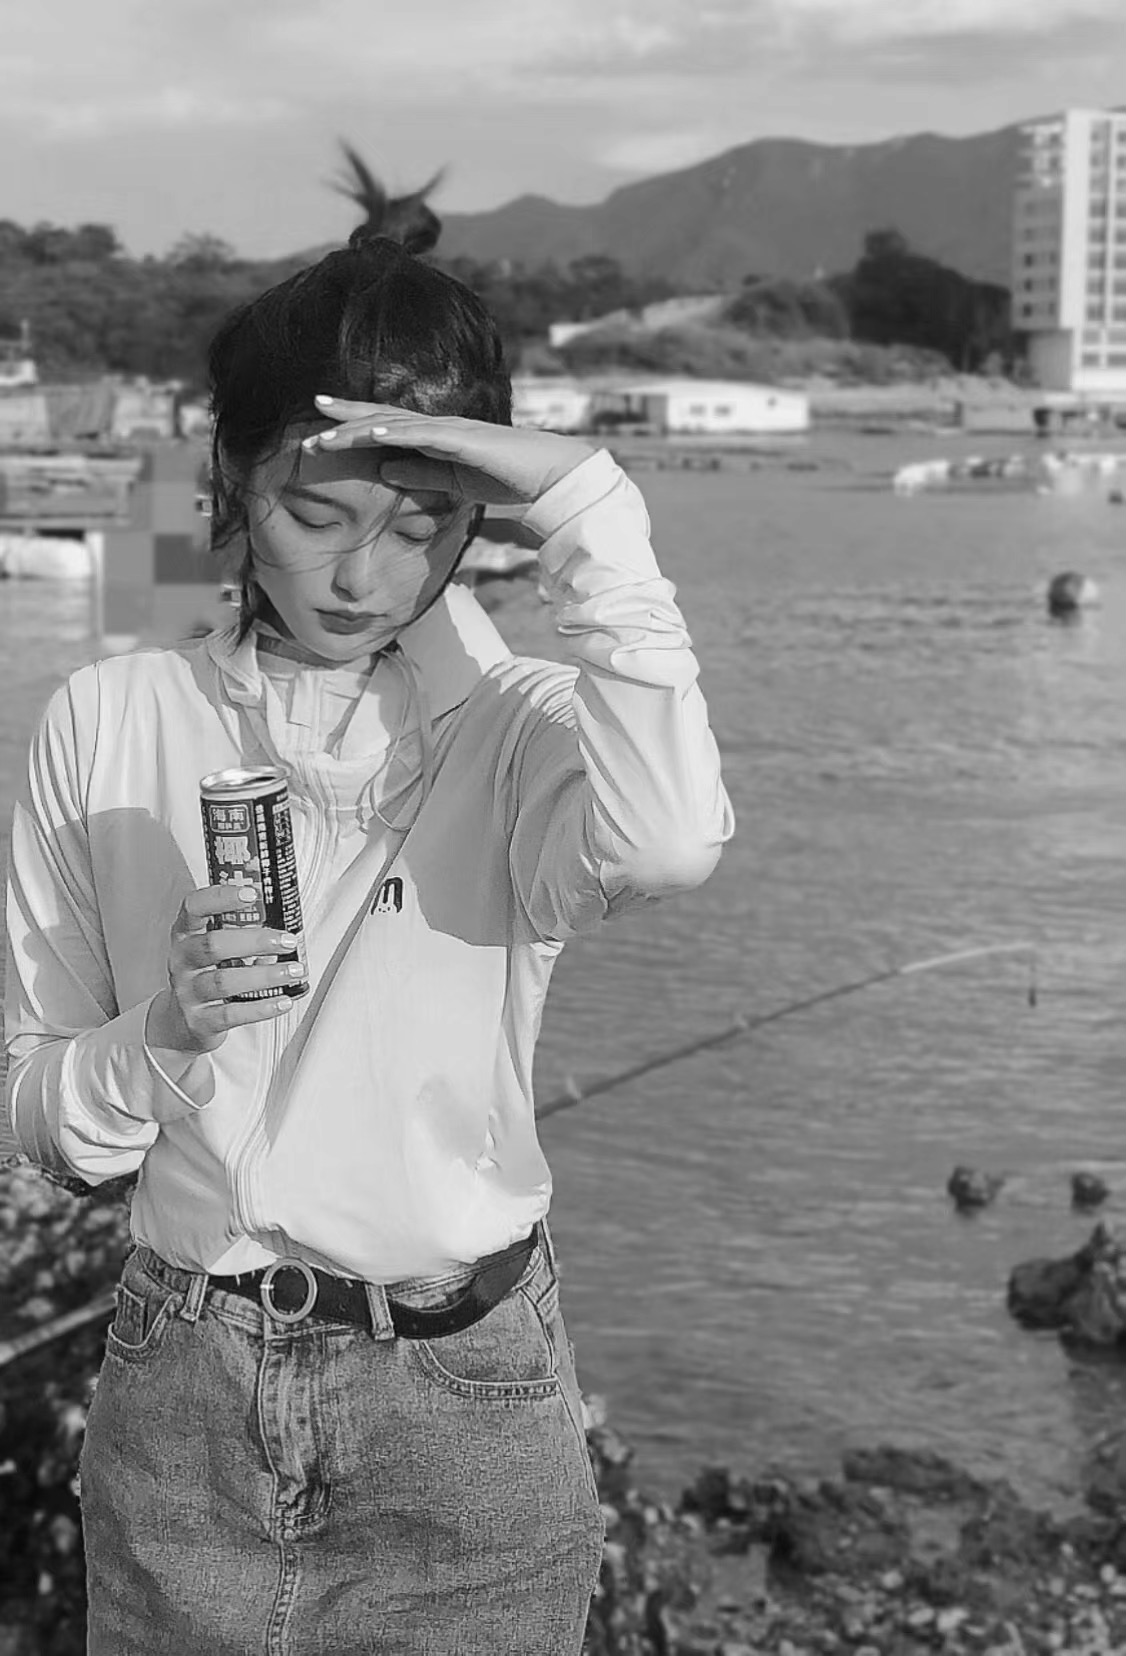
\includegraphics[width=5.5cm,height=8cm]{xuan1.png}
                \caption{转化成灰度图像之后的图像}
                \end{figure}
  \subsubsection{调用python \quad cv2函数库里的函数,进行直方图均衡化}

  如图
  \begin{figure}[h!]
                \centering
                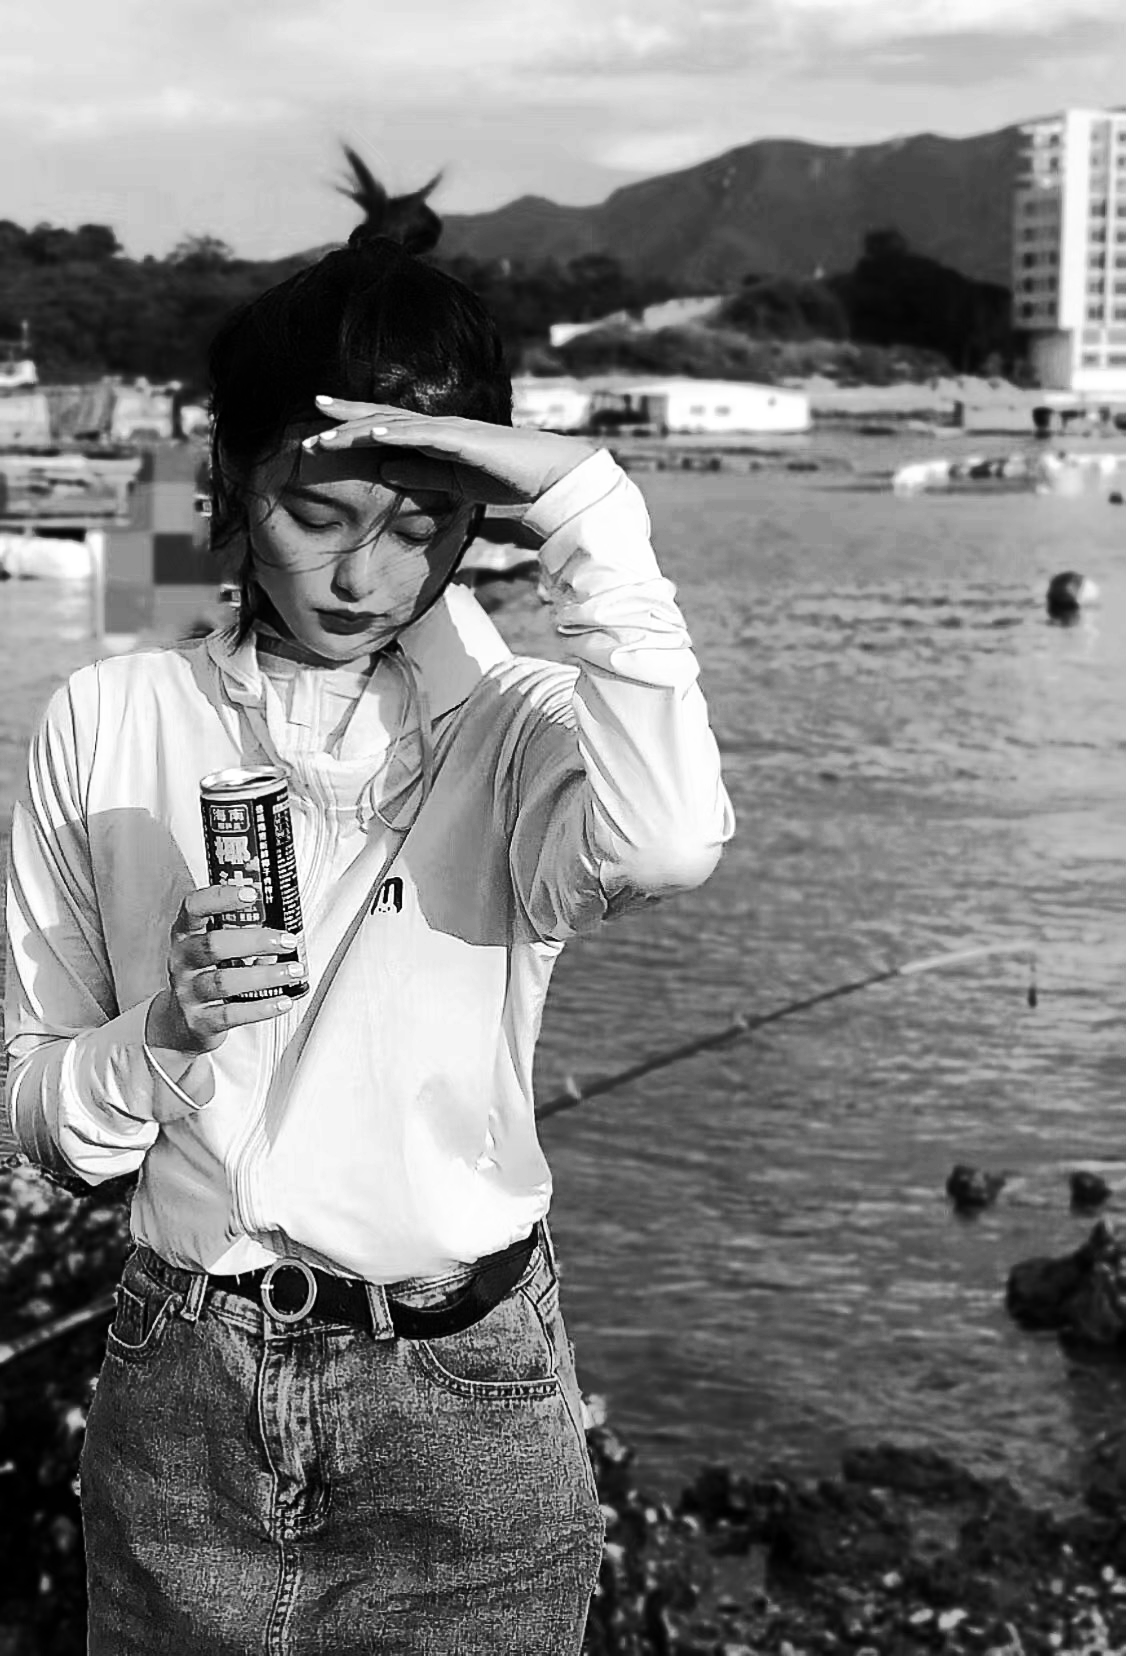
\includegraphics[width=5.5cm,height=8cm]{xuan2.png}
                \caption{库函数直方图均衡化的图像}
                \end{figure}
  \subsubsection{自己手动编程实现直方图均衡化}
  \begin{enumerate}
    \item 统计各灰度值出现的次数
    \item 计算各灰度值出现的频率$$r_i=\frac{n_i}{n}$$
    \item 求累计分布函数 $$s_k=\sum_{i=0}^{k} r_i$$
    \item 进行取整扩展 $$s'_i=\left \lfloor s_i*255+0.5 \right \rfloor$$
    \item 输出处理后的图像

    如图
     \begin{figure}[h!]
                \centering
                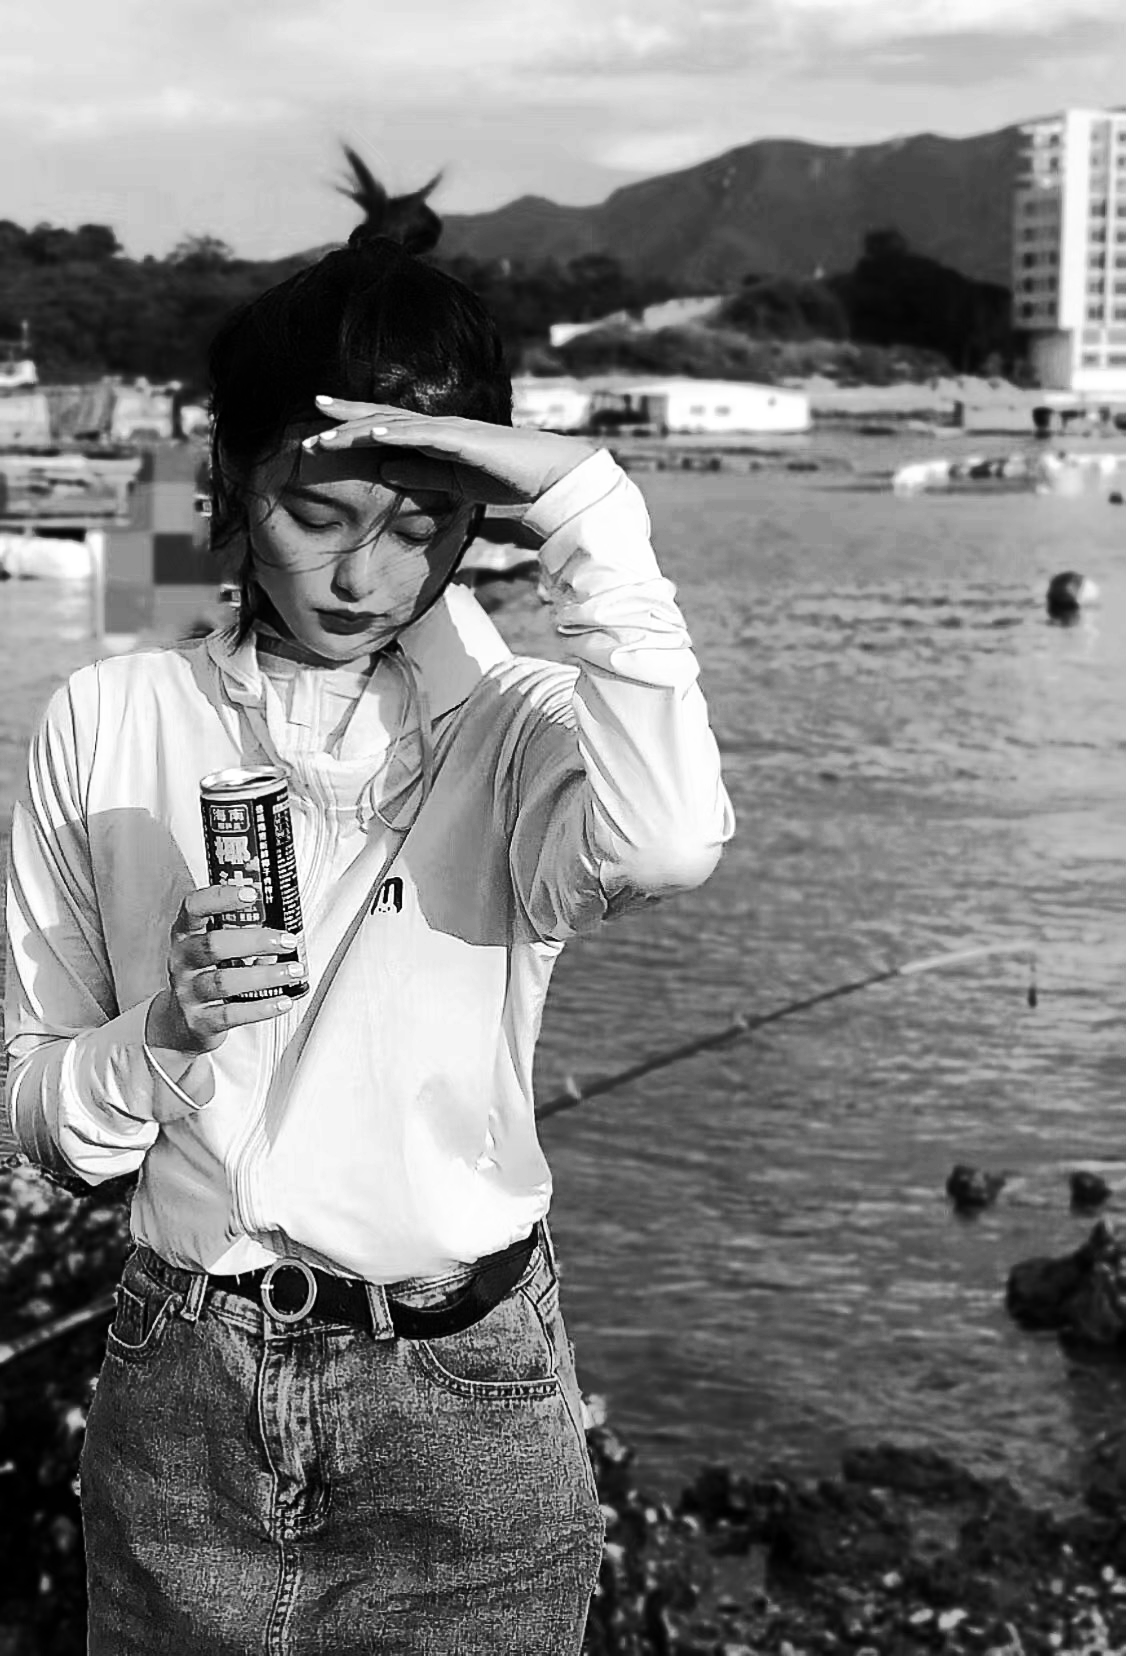
\includegraphics[width=5.5cm,height=8cm]{xuan3.png}
                \caption{自己写的函数直方图均衡化的图像}
                \end{figure}
  \end{enumerate}
 \newpage
  \subsubsection{进行对比检查,用自己写的函数处理之后的图像与库函数处理之后的图像进行对比}

  将两幅图像做差
  \begin{figure}[h!]
                \centering
                
\includegraphics[width=5.5cm,height=8cm]{xuan4.png}
                \caption{两幅图像做差之后的结果图像}
                \end{figure}
   \subsubsection{输出灰度频率直方图}

   统计次数、计算频率、求累计分布函数、取整扩展确定映射关系计算概率
   \begin{figure}[h!]
                \centering
                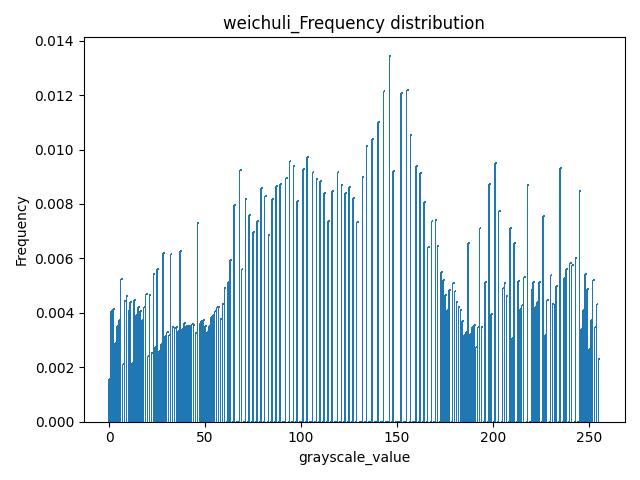
\includegraphics[width=10cm,height=7.9cm]{xuan6.png}
                \caption{原始图像灰度频率直方图}
                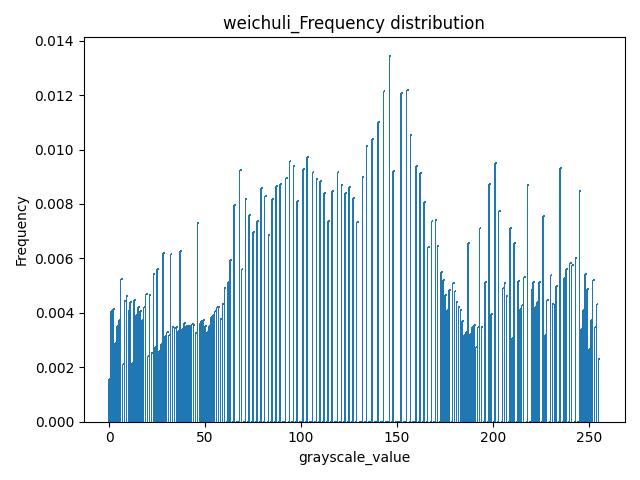
\includegraphics[width=10cm,height=7.9cm]{xuan6.png}
                \caption{调用库函数处理之后图像频率直方图}
                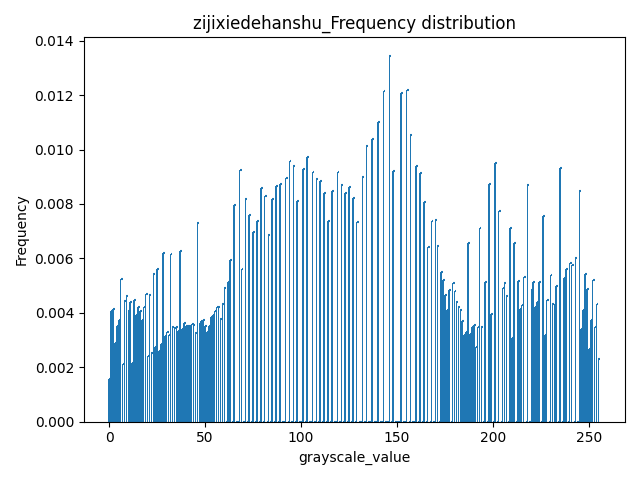
\includegraphics[width=10cm,height=7.9cm]{xuan7.png}
                \caption{自己写的函数处理之后图像灰度频率直方图}
                \end{figure}
\clearpage
\newpage
\subsection{编程语言的注释说明}
\begin{python}
from cv2 import cv2
import numpy as np
from matplotlib import pyplot as plt


def My_equalizeHist(I):
    rows, cols = I.shape

    # 统计各级灰度出现的次数
    hist1 = np.zeros(256)
    for r in range(rows):
        for c in range(cols):
            hist1[I[r][c]] += 1

    # 求累积直方图
    sum = 0
    for i in range(256):
        sum += hist1[i] / (rows * cols)
        hist1[i] = sum

    # 求均衡化的像素值
    newI = np.zeros((rows, cols), np.uint8)
    for i in range(rows):
        for j in range(cols):
            newI[i][j] = (np.uint8)(255 * hist1[I[i][j]] + 0.5)
    return newI


def output(a, s):
    rows, cols = a.shape

    # 统计各级灰度出现的次数
    hist1 = np.zeros(256)
    hist2 = np.zeros(256)
    for r in range(rows):
        for c in range(cols):
            hist1[a[r][c]] += 1

    # 求累积直方图
    sum = 0
    for i in range(256):
        hist2[i] = hist1[i] / (rows * cols)
        sum += hist2[i]
        hist1[i] = sum
        
    # 求均衡化的像素值
    res = np.zeros(256)
    for i in range(256):
        res[(np.uint8)(255 * hist1[i] + 0.5)] += hist2[i]
        
    # 画出频率直方图
    x = [x for x in range(256)]
    plt.bar(x, res, align='center')
    plt.xlabel('grayscale_value')
    plt.ylabel('Frequency')
    plt.title(s)
    for i in range(len(res)):
        plt.hlines(res[i], x[i], x[i] + 1)
    plt.show()


def check(a, b):
    #两者做差
    rows, cols = a.shape
    res = np.zeros((rows, cols), np.uint8)
    for i in range(rows):
        for j in range(cols):
            res[i][j] = a[i][j] - b[i][j]
    cv2.imwrite("xuan4.png", res)


if __name__ == "__main__":
    img = cv2.imread("xuan.png")  # 读入图像

    img = cv2.cvtColor(img, cv2.COLOR_BGR2GRAY)  # 把彩色图像换成灰度图像
    cv2.imwrite("xuan1.png", img)  # 输出灰度图像
    output(img, "weichuli_Frequency distribution")

    hist = cv2.equalizeHist(img)  # 调用cv中直方图均衡化函数
    cv2.imwrite("xuan2.png", hist)  # 输出调用cv中均衡化函数之后的图像
    output(hist, "diaoyonghanshu_Frequency distribution")

    hist1 = My_equalizeHist(img)  # 调用自己写的均衡化函数
    cv2.imwrite("xuan3.png", hist1)  # 输出调用自己写的均衡化函数之后的图像
    output(hist1, "zijixiedehanshu_Frequency distribution")

    check(hist, hist1)
    '''
    对调用cv中函数与自己写的函数区别,输出的图像越黑,说明两者越相近
    '''


\end{python}
\subsection{所需的软件、环境、函数库名}

\begin{enumerate}
    \item 软件:pycharm
    \item 环境:windows10、python3
    \item 函数库名
    \begin{figure}[h!]
                \centering
                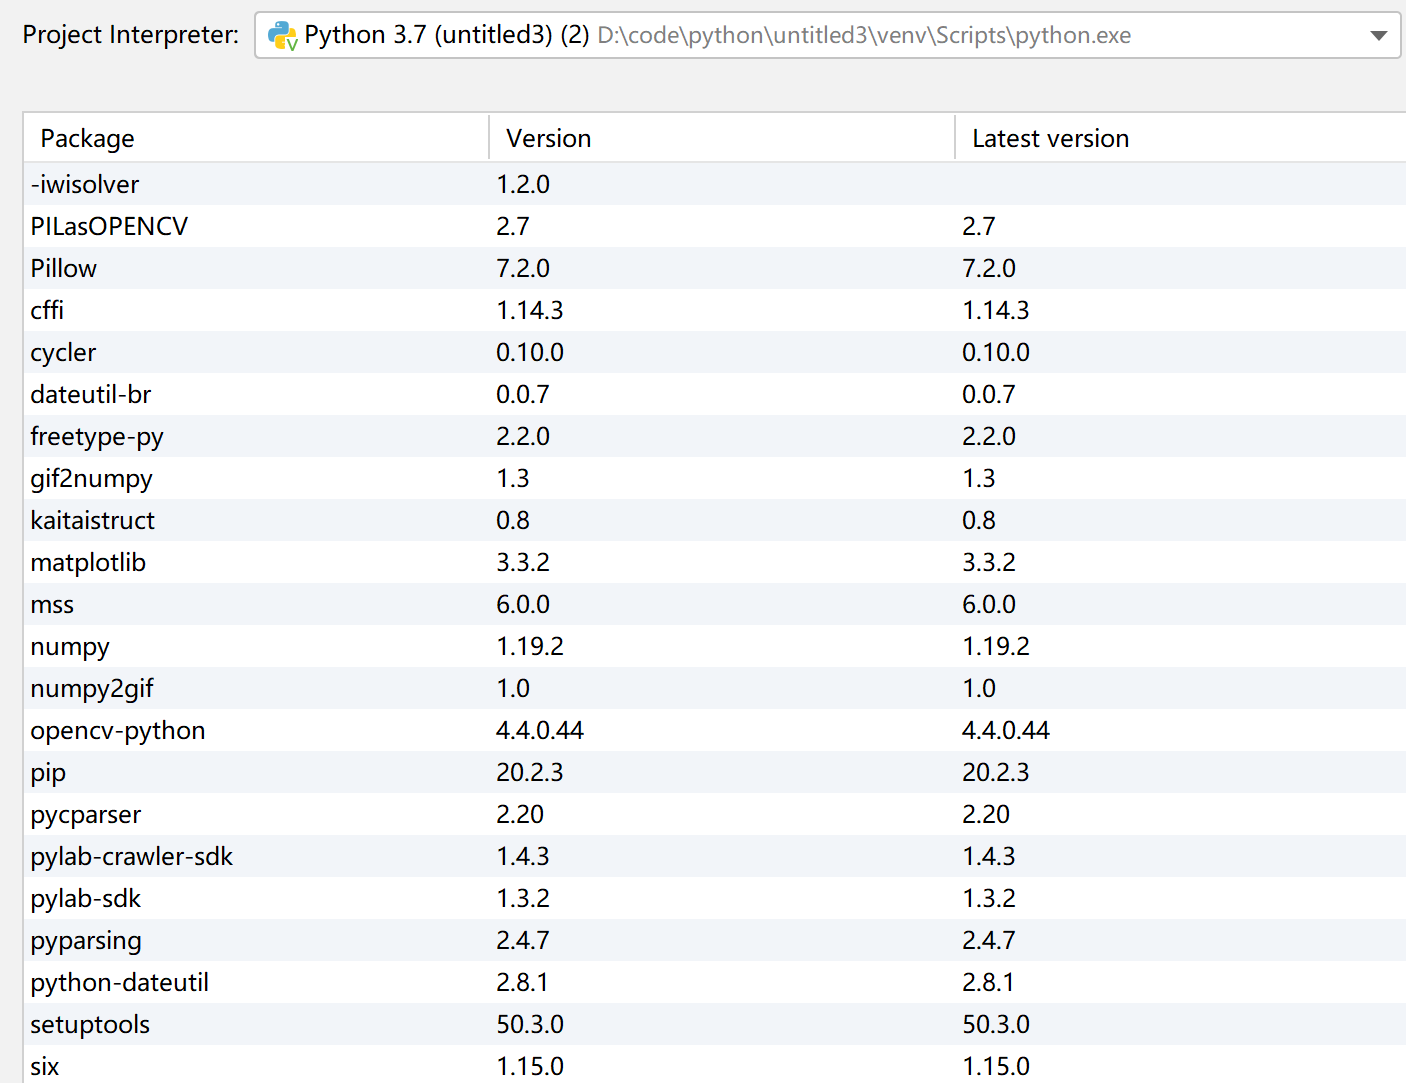
\includegraphics[width=14cm,height=9cm]{python.png}

\vskip 12cm
    \end{figure}

\end{enumerate}
\clearpage
\newpage
\section{直方图规定化}
\subsection{SML}
\subsection{代码编写的简单思路}
\subsubsection{挑选一张合适的原始图像、一张参考图像}

  如图
                \begin{figure}[h!]
                \centering
                
\includegraphics[width=5.5cm,height=8cm]{xuan9.png}
                \caption{原始图像}
                \end{figure}
                \begin{figure}[h!]
                \centering
                
\includegraphics[width=5.5cm,height=8cm]{xuan8.png}
                \caption{参考图像}
                \end{figure}

  \subsubsection{先读入原始图像、参考图像,转化成灰度图像,输出原始的灰度图像、参考的灰度图像}

  如图
  \begin{figure}[h!]
                \centering
                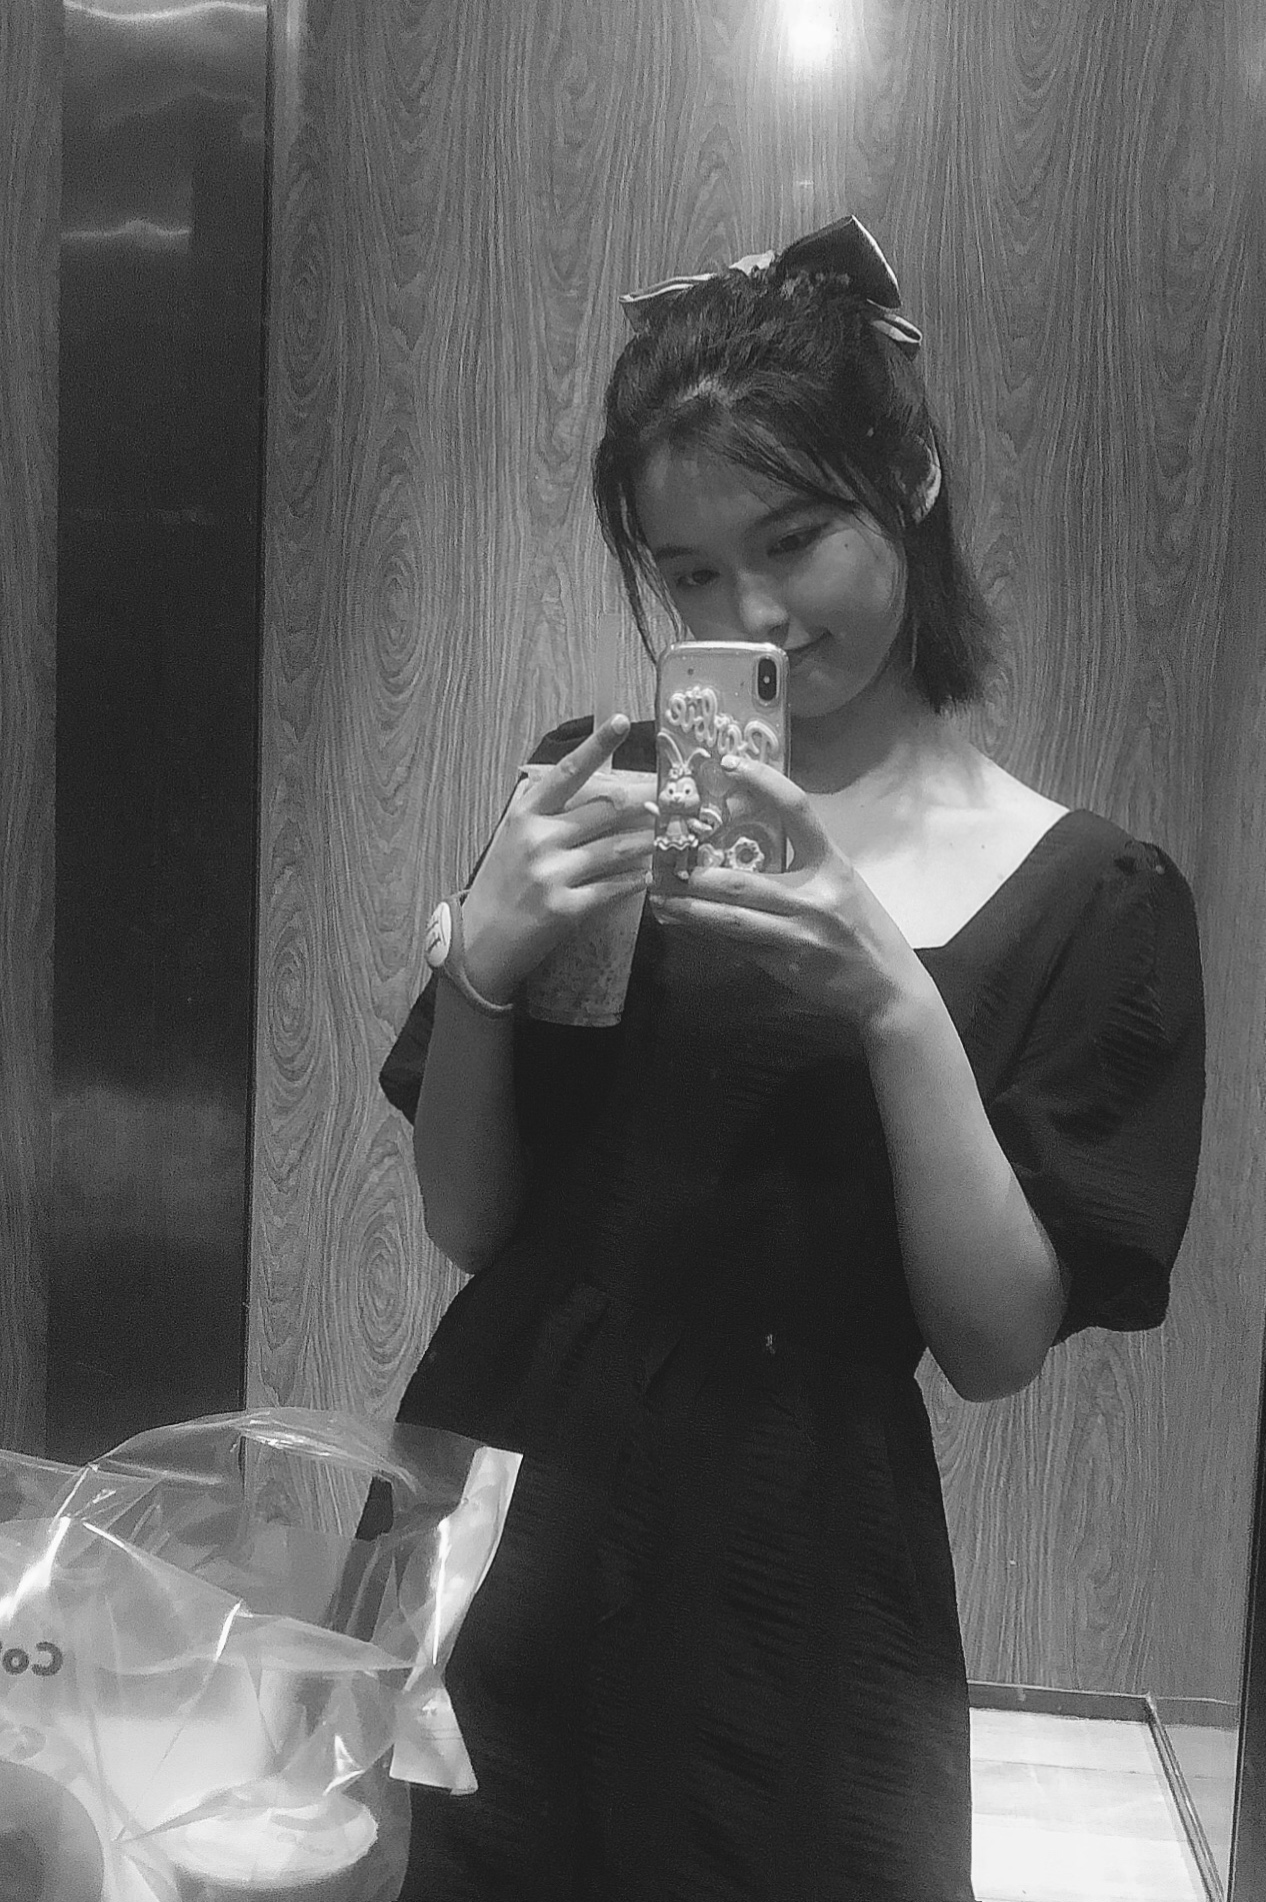
\includegraphics[width=5.5cm,height=8cm]{xuan10.png}
                \caption{原始转化成灰度图像之后的图像}
                \end{figure}
  \begin{figure}[h!]
                \centering
                
\includegraphics[width=5.5cm,height=8cm]{xuan11.png}
                \caption{参考转化成灰度图像之后的图像}
                \end{figure}
  \subsubsection{自己手动编程实现直方图规定化}
  \begin{enumerate}
    \item 分别对原始图像、参考图像计算累计直方图
    $$s_{k}=\sum_{j=0}^{k} \frac{n_{j}}{n}$$

    $$v_{k}=G(z_{k})=\sum_{i=0}^{k} p_{z}(z_i)$$
对一个$s_k$值计算满足$G(z_{k})-s_{k}=0$最接近的整数$z_k$
原始图像的每个像素$r_k$,将该值映射到其对应的灰度
级$s_k$;然后映射灰度级$s_k$到最终灰度级$z_k$

    \subsubsection{输出规定化图像}
    如图
     \begin{figure}[h!]
                \centering
                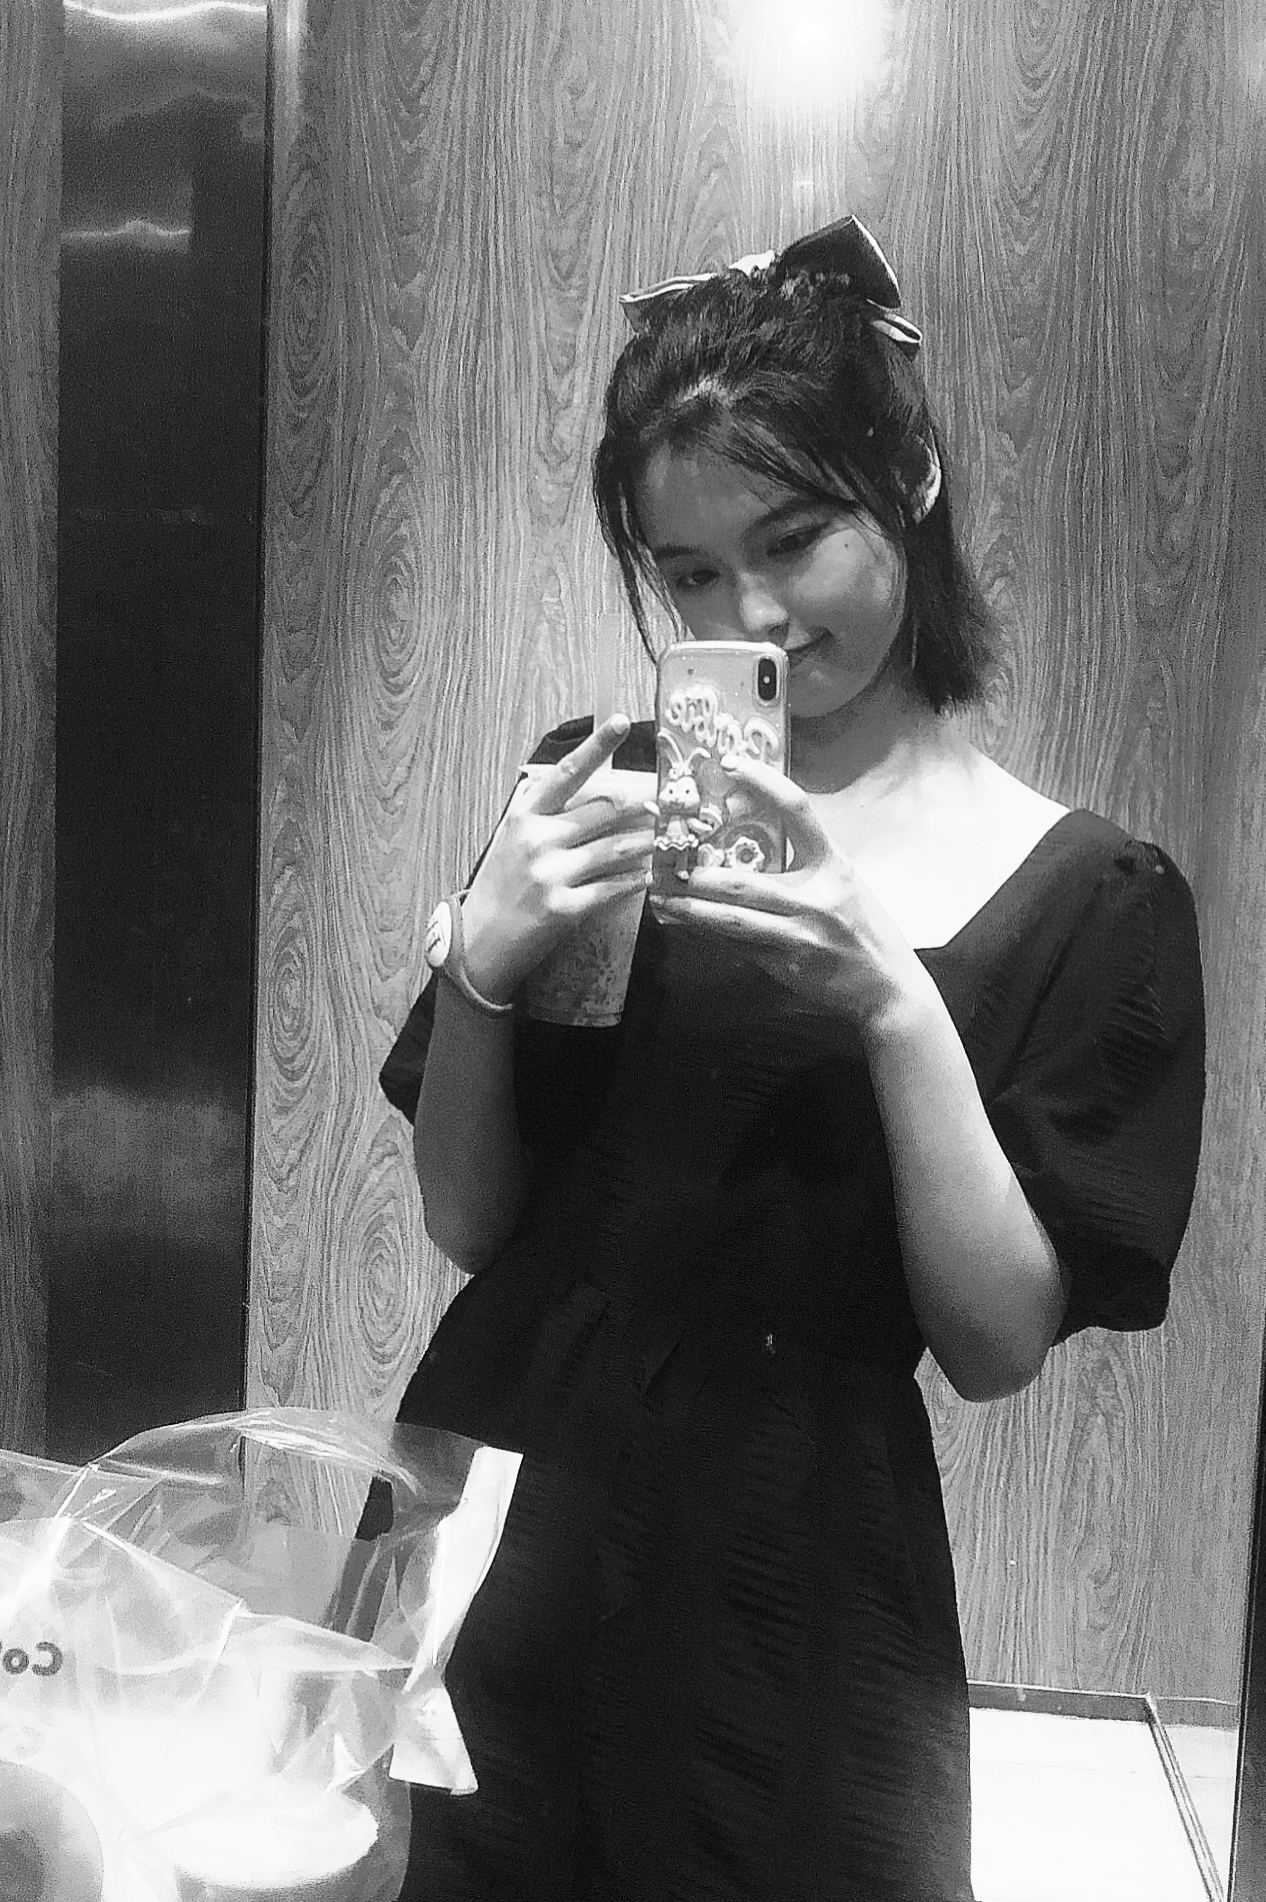
\includegraphics[width=5.5cm,height=8cm]{xuan12.png}
                \caption{自己写的函数直方图规定化的图像}
                \end{figure}
  \end{enumerate}
   \subsubsection{输出灰度频率直方图}

   统计次数、计算频率、求累计分布函数、取整扩展确定映射关系计算概率
   \begin{figure}[h!]
                \centering
                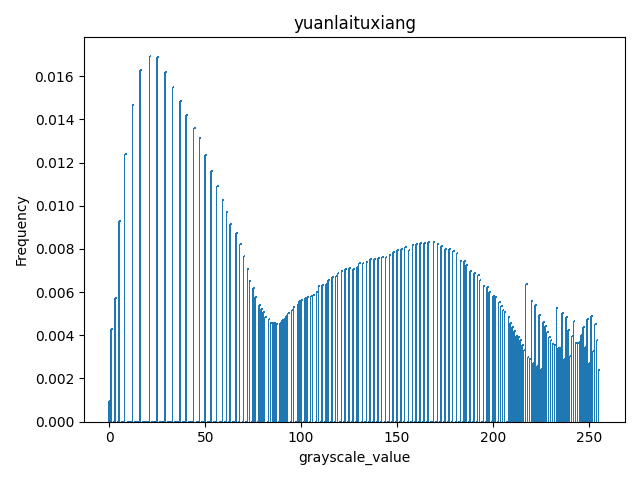
\includegraphics[width=10cm,height=7.9cm]{xuan20.png}
                \caption{原始图像灰度频率直方图}
                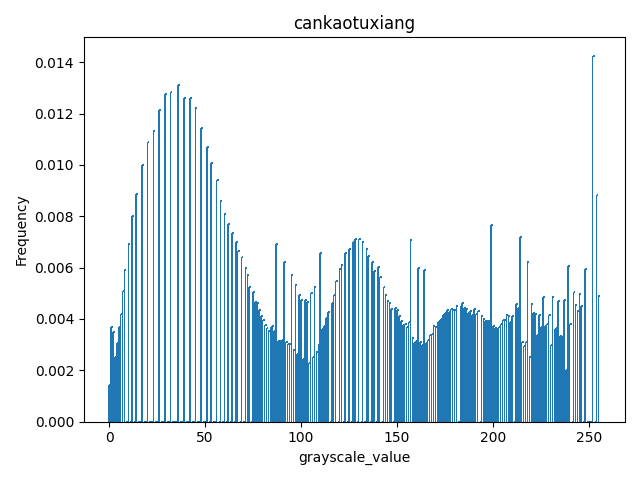
\includegraphics[width=10cm,height=7.9cm]{xuan30.png}
                \caption{参考图像灰度频率直方图}
                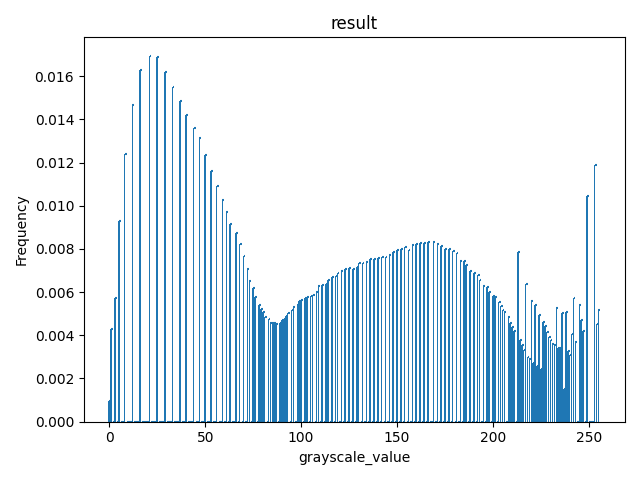
\includegraphics[width=10cm,height=7.9cm]{xuan40.png}
                \caption{自己写的函数处理之后图像灰度频率直方图}
                \end{figure}
\clearpage
\newpage
\subsection{编程语言的注释说明}
\begin{python}
import numpy as np
import matplotlib.pyplot as plt
import cv2

def My_equalizeHist(I):
    rows, cols = I.shape

    # 统计各级灰度出现的次数
    hist = np.zeros(256, dtype=np.float32)
    for r in range(rows):
        for c in range(cols):
            hist[I[r][c]] += 1

    # 求累积直方图
    sum = 0
    for i in range(256):
        sum += hist[i] / (rows * cols)
        hist[i] = sum
    return hist

# 定义函数,直方图规定化
def histSpecification(a, b):  # specification image and reference image
    a1 = My_equalizeHist(a)  # 计算待匹配直方图
    b1 = My_equalizeHist(b)  # 计算参考直方图
    res = np.zeros(256, dtype=np.uint8)  # correspond value
    # 直方图规定化
    for i in range(256):
        d = np.abs(a1[i] - b1[i])
        k = i
        for j in range(256):
            if np.abs(a1[i] - b1[j]) < d:
                d = np.abs(a1[i] - b1[j])
                k = j
        res[i] = k
    return cv2.LUT(a, res)


def output(a, s):
    rows, cols = a.shape

    # 统计各级灰度出现的次数
    hist1 = np.zeros(256)
    hist2 = np.zeros(256)
    for r in range(rows):
        for c in range(cols):
            hist1[a[r][c]] += 1

    # 求累积直方图
    sum = 0
    for i in range(256):
        hist2[i] = hist1[i] / (rows * cols)
        sum += hist2[i]
        hist1[i] = sum

    # 求均衡化的像素值
    res = np.zeros(256)
    for i in range(256):
        res[(np.uint8)(255 * hist1[i] + 0.5)] += hist2[i]

    # 画出频率直方图
    x = [x for x in range(256)]
    plt.bar(x, res, align='center')
    plt.xlabel('grayscale_value')
    plt.ylabel('Frequency')
    plt.title(s)
    for i in range(len(res)):
        plt.hlines(res[i], x[i], x[i] + 1)
    plt.show()

if __name__ == "__main__":
    img = cv2.imread('xuan1.png', cv2.IMREAD_GRAYSCALE)
    # 读入参考图像
    img1 = cv2.imread('xuan5.png', cv2.IMREAD_GRAYSCALE)
    cv2.imwrite('xuan2.png', img)
    output(img,"yuanlaituxiang")
    cv2.imwrite('xuan3.png', img1)
    output(img1,"cankaotuxiang")
    img2 = histSpecification(img, img1)
    cv2.imwrite('xuan4.png', img2)
    output(img2,"result")

\end{python}
\subsection{所需的软件、环境、函数库名}

\begin{enumerate}
    \item 软件:pycharm
    \item 环境:windows10、python3
    \item 函数库名
    \begin{figure}[h!]
                \centering
                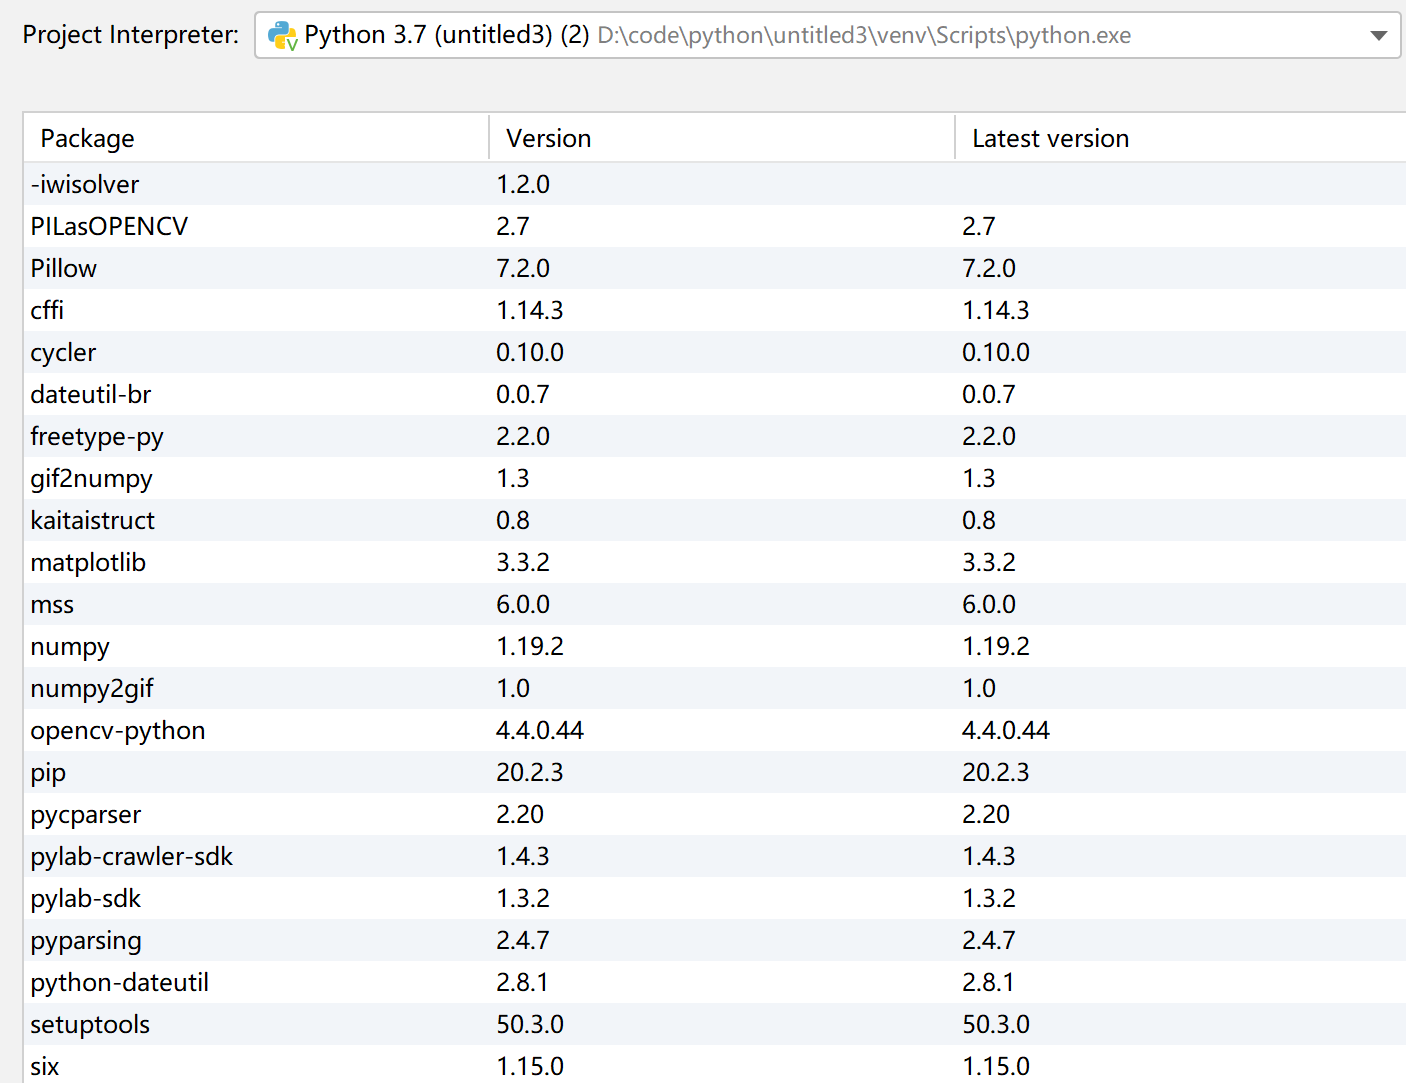
\includegraphics[width=14cm,height=9cm]{python.png}
    \end{figure}
\end{enumerate}
\subsection{GML}
\subsection{代码编写的简单思路}
\subsubsection{挑选一张合适的原始图像、一张参考图像}

  如图
                \begin{figure}[h!]
                \centering
                
\includegraphics[width=5.5cm,height=8cm]{xuan9.png}
                \caption{原始图像}
                \end{figure}
                \begin{figure}[h!]
                \centering
                
\includegraphics[width=5.5cm,height=8cm]{xuan8.png}
                \caption{参考图像}
                \end{figure}

  \subsubsection{先读入原始图像、参考图像,转化成灰度图像,输出原始的灰度图像、参考的灰度图像}

  如图
  \begin{figure}[h!]
                \centering
                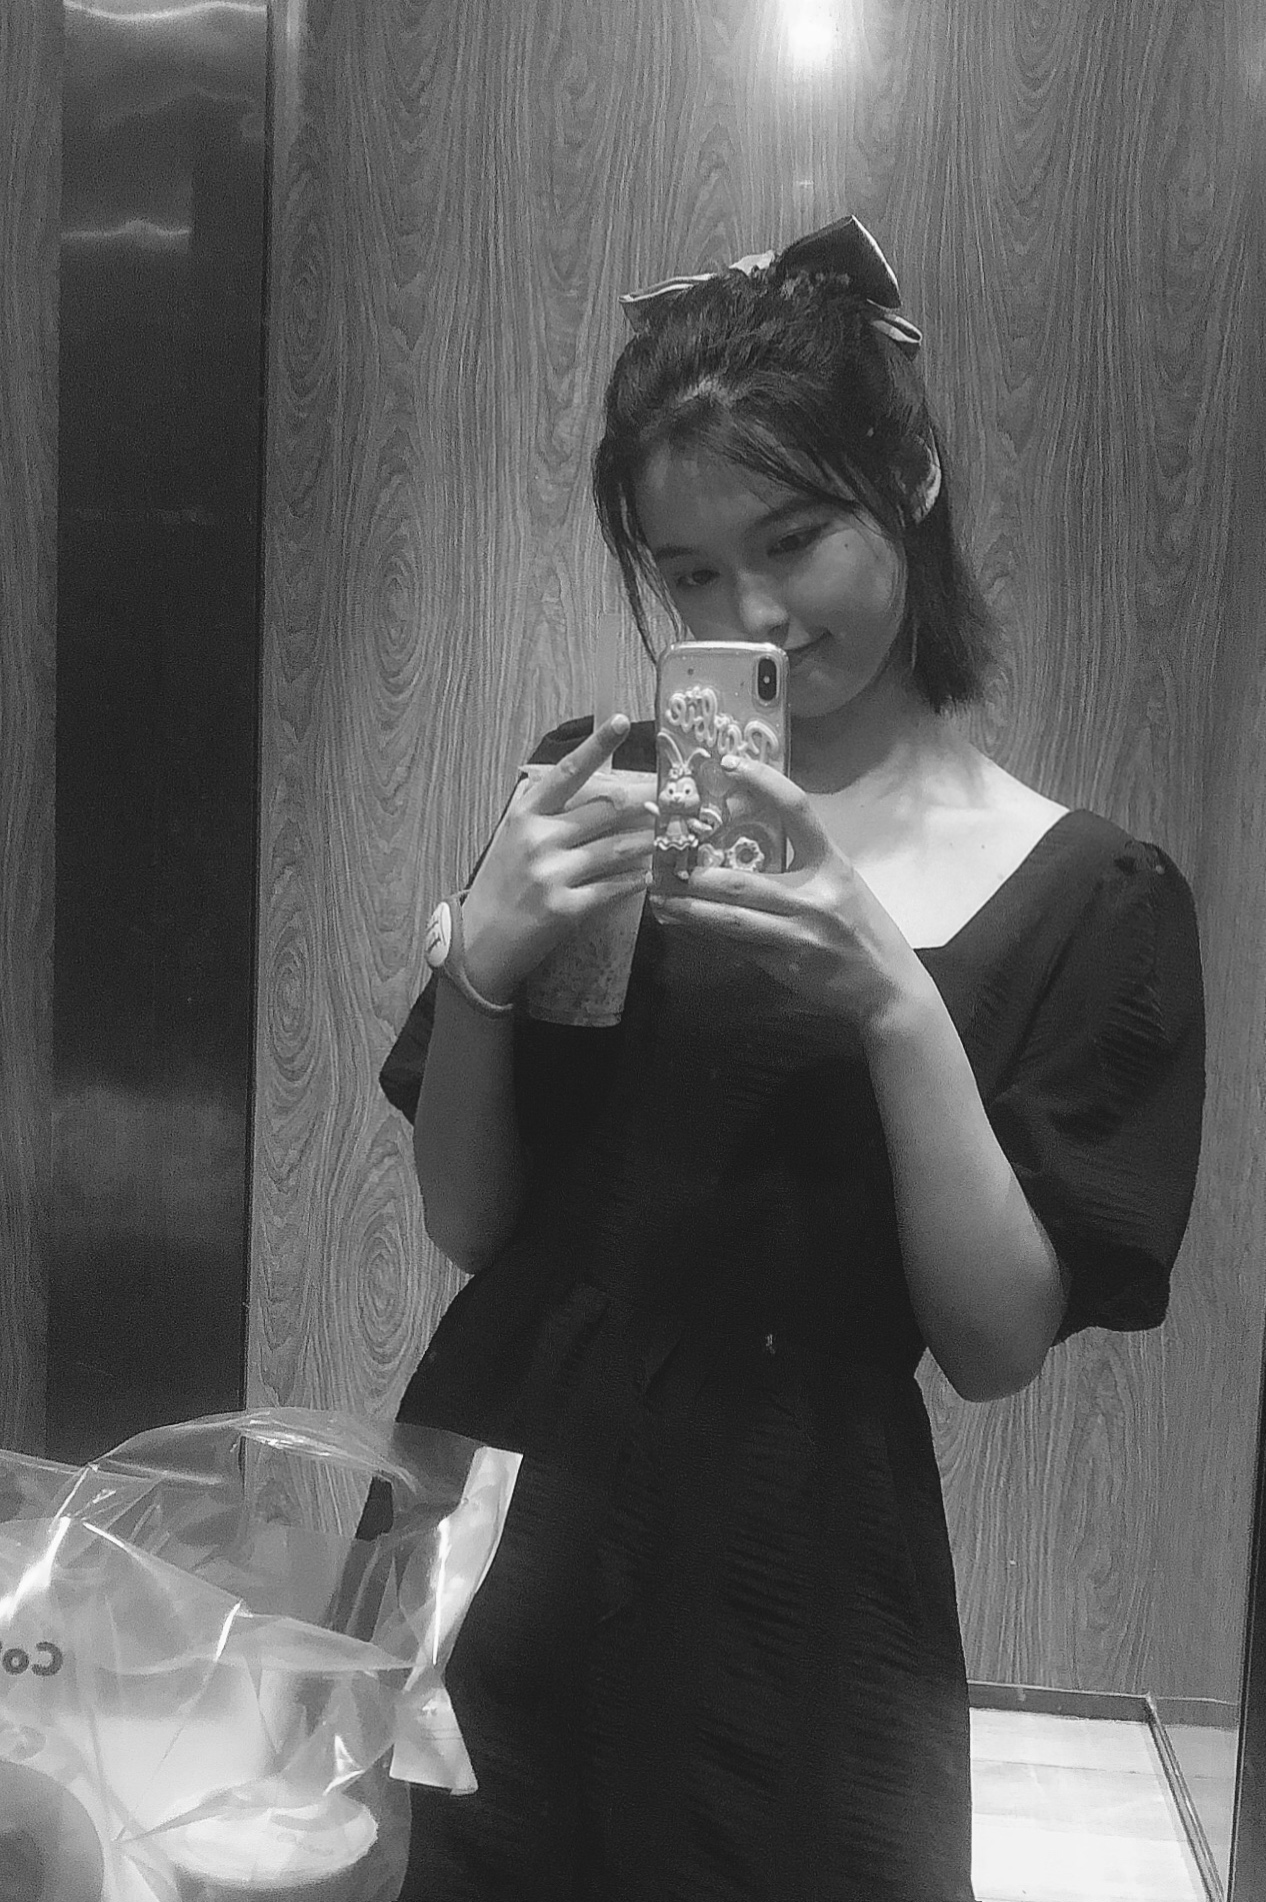
\includegraphics[width=5.5cm,height=8cm]{xuan10.png}
                \caption{原始转化成灰度图像之后的图像}
                \end{figure}
  \begin{figure}[h!]
                \centering
                
\includegraphics[width=5.5cm,height=8cm]{xuan11.png}
                \caption{参考转化成灰度图像之后的图像}
                \end{figure}
  \subsubsection{自己手动编程实现直方图规定化}
  \begin{enumerate}
    \item 分别对原始图像、参考图像计算累计直方图
    $$s_{k}=\sum_{j=0}^{k} \frac{n_{j}}{n}$$

    $$v_{k}=G(z_{k})=\sum_{i=0}^{k} p_{z}(z_i)$$
% 对一个$s_k$值计算满足$G(z_{k})-s_{k}=0$最接近的整数$z_k$
% 原始图像的每个像素$r_k$,将该值映射到其对应的灰度
% 级$s_k$;然后映射灰度级$s_k$到最终灰度级$z_k$

    \subsubsection{输出规定化图像}
    如图
     \begin{figure}[h!]
                \centering
                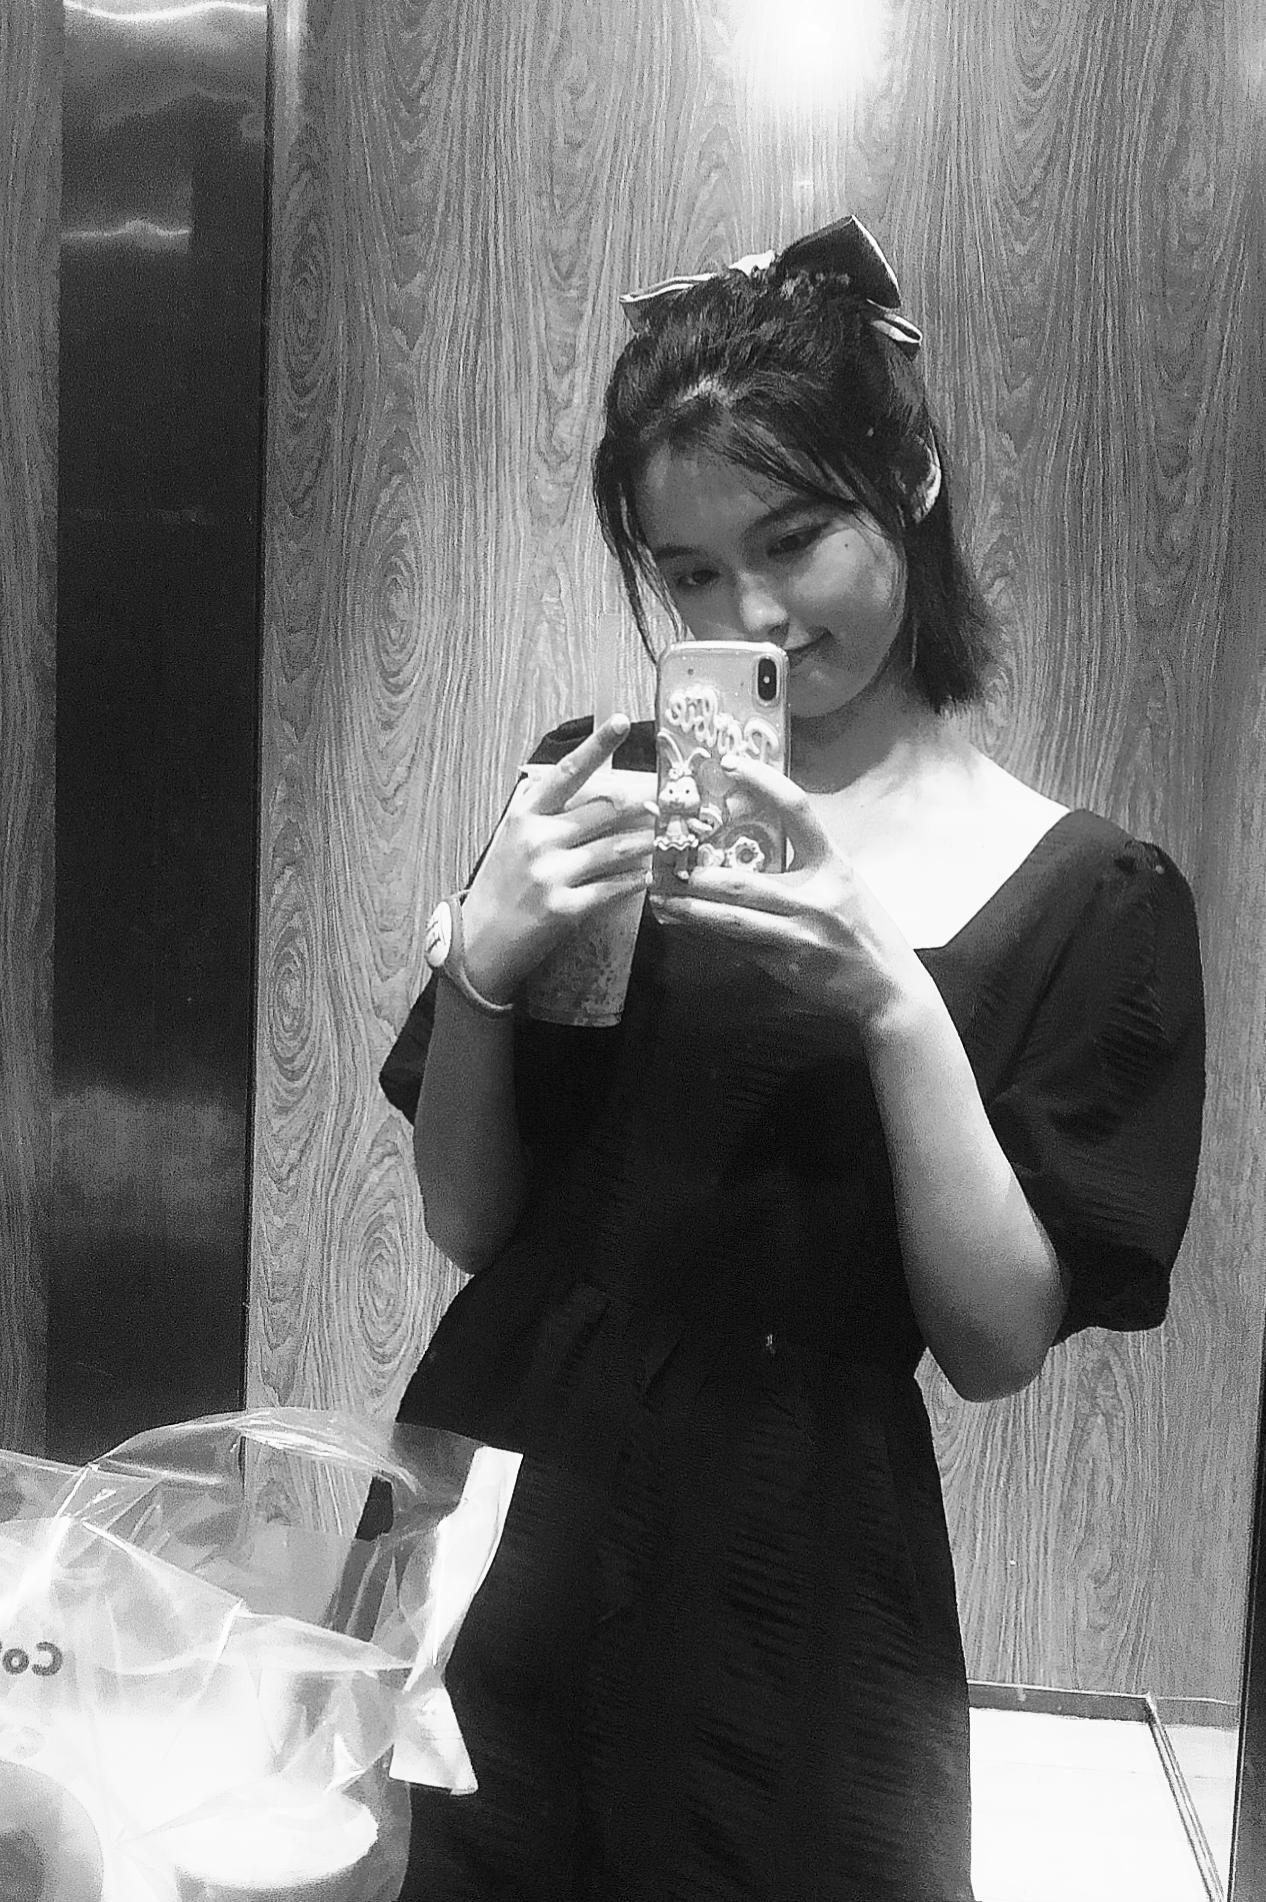
\includegraphics[width=5.5cm,height=8cm]{xuan15.png}
                \caption{自己写的函数直方图规定化的图像}
                \end{figure}
  \end{enumerate}
   \subsubsection{输出灰度频率直方图}

   统计次数、计算频率、求累计分布函数、取整扩展确定映射关系计算概率
   \begin{figure}[h!]
                \centering
                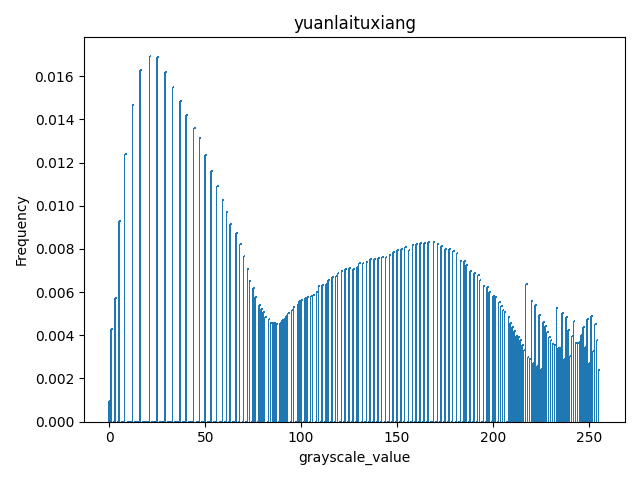
\includegraphics[width=10cm,height=7.9cm]{xuan20.png}
                \caption{原始图像灰度频率直方图}
                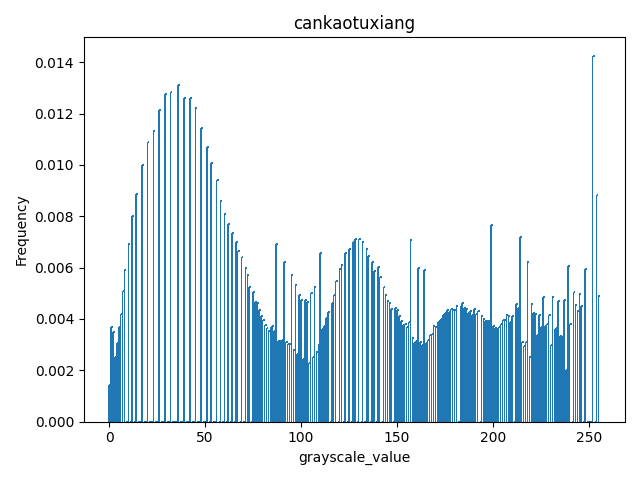
\includegraphics[width=10cm,height=7.9cm]{xuan30.png}
                \caption{参考图像灰度频率直方图}
                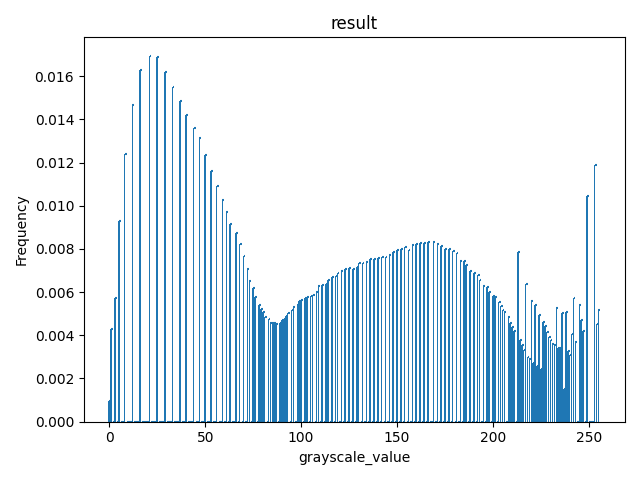
\includegraphics[width=10cm,height=7.9cm]{xuan50.png}
                \caption{自己写的函数处理之后图像灰度频率直方图}
                \end{figure}
\clearpage
\newpage
\subsection{编程语言的注释说明}
\begin{python}
import numpy as np
import matplotlib.pyplot as plt
import cv2

def My_equalizeHist(I):
    rows, cols = I.shape

    # 统计各级灰度出现的次数
    hist = np.zeros(256, dtype=np.float32)
    for r in range(rows):
        for c in range(cols):
            hist[I[r][c]] += 1

    # 求累积直方图
    sum = 0
    for i in range(256):
        sum += hist[i] / (rows * cols)
        hist[i] = sum
    return hist

# 定义函数,直方图规定化
def histSpecification(a, b):  # specification image and reference image
    a1 = My_equalizeHist(a)  # 计算待匹配直方图
    b1 = My_equalizeHist(b)  # 计算参考直方图
    res = np.zeros(256, dtype=np.uint8)  # correspond value
    dis = np.zeros((256,256), dtype=np.float32)
    # 直方图规定化
    # GML
    for y in range(256):
        for x in range(256):
            dis[x][y]=np.abs(a1[y]-b1[x])
    last=0
    laen=0
    st=0
    en=0
    for x in range(256):
        d=dis[x][0]
        for y in range(256):
            if (d>dis[x][y]):
                en=y
                d=dis[x][y]

        if (st!=last or en!=laen):
            for i in range(st,en+1):
                res[i]=x
            last=st
            laen=en
            st=laen+1

    return cv2.LUT(a,res)

def output(a, s):
    rows, cols = a.shape

    # 统计各级灰度出现的次数
    hist1 = np.zeros(256)
    hist2 = np.zeros(256)
    for r in range(rows):
        for c in range(cols):
            hist1[a[r][c]] += 1

    # 求累积直方图
    sum = 0
    for i in range(256):
        hist2[i] = hist1[i] / (rows * cols)
        sum += hist2[i]
        hist1[i] = sum

    # 求均衡化的像素值
    res = np.zeros(256)
    for i in range(256):
        res[(np.uint8)(255 * hist1[i] + 0.5)] += hist2[i]

    # 画出频率直方图
    x = [x for x in range(256)]
    plt.bar(x, res, align='center')
    plt.xlabel('grayscale_value')
    plt.ylabel('Frequency')
    plt.title(s)
    for i in range(len(res)):
        plt.hlines(res[i], x[i], x[i] + 1)
    plt.show()

if __name__ == "__main__":
    img = cv2.imread('xuan1.png', cv2.IMREAD_GRAYSCALE)
    # 读入参考图像
    img1 = cv2.imread('xuan5.png', cv2.IMREAD_GRAYSCALE)
    cv2.imwrite('xuan2.png', img)
    output(img,"yuanlaituxiang")
    cv2.imwrite('xuan3.png', img1)
    output(img1,"cankaotuxiang")
    img2 = histSpecification(img, img1)
    cv2.imwrite('xuan4.png', img2)
    output(img2,"result")

\end{python}
\subsection{所需的软件、环境、函数库名}

\begin{enumerate}
    \item 软件:pycharm
    \item 环境:windows10、python3
    \item 函数库名
    \begin{figure}[h!]
                \centering
                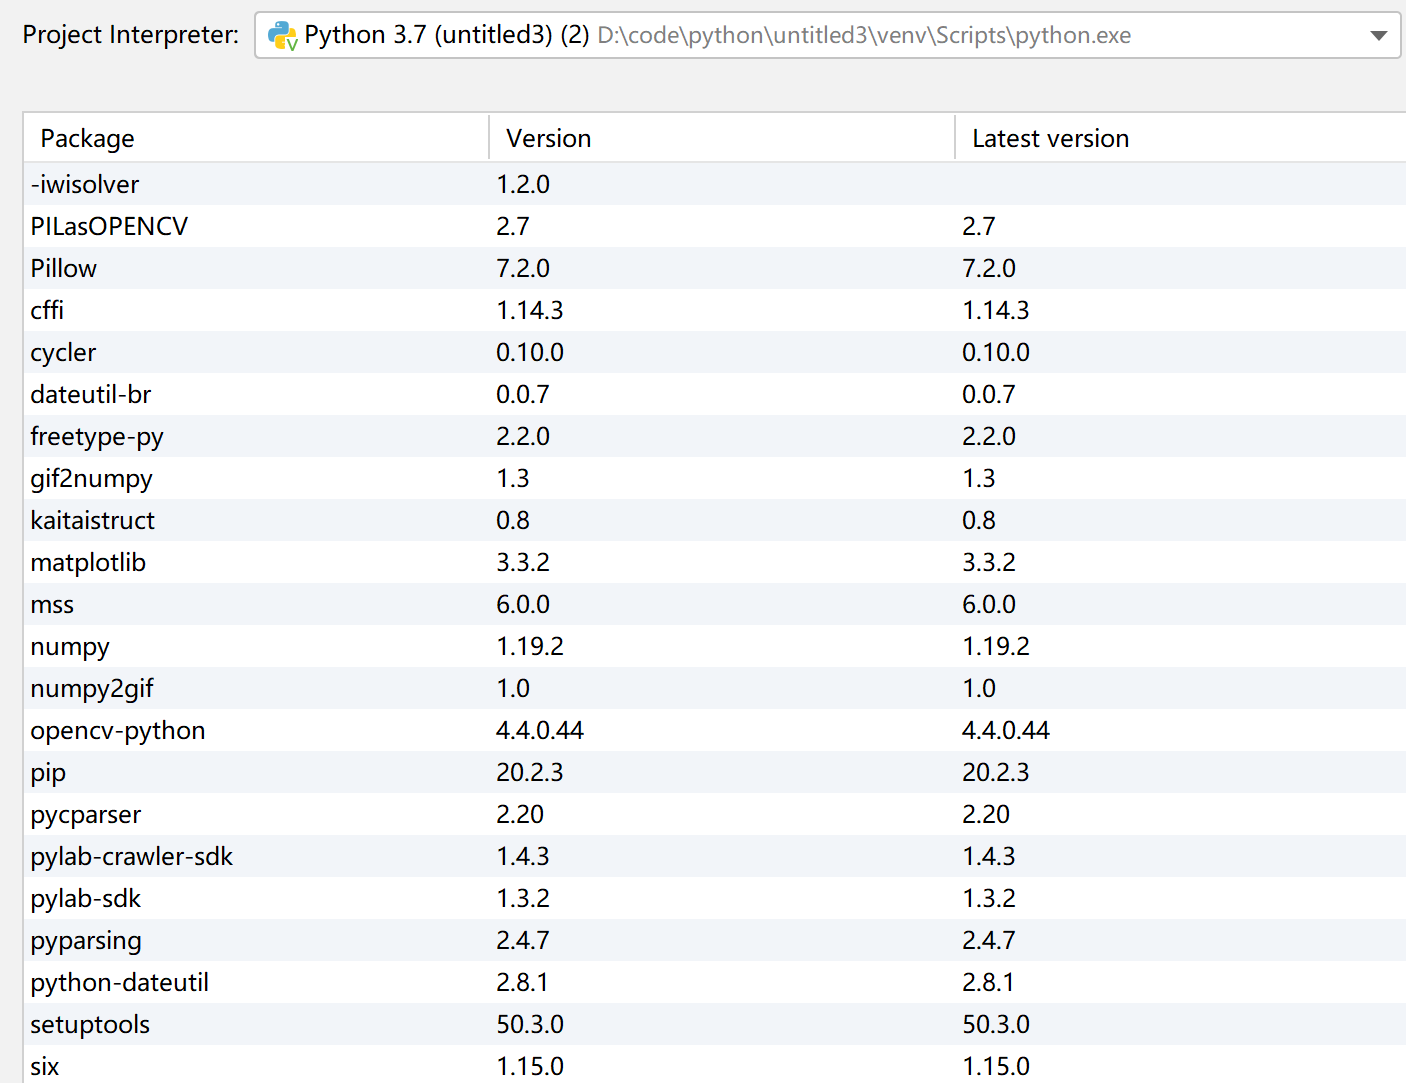
\includegraphics[width=14cm,height=9cm]{python.png}
    \end{figure}
\end{enumerate}
\newpage
\subsection{SML与GML区别}
做差,越黑说明越相同
\begin{figure}[h!]
                \centering
                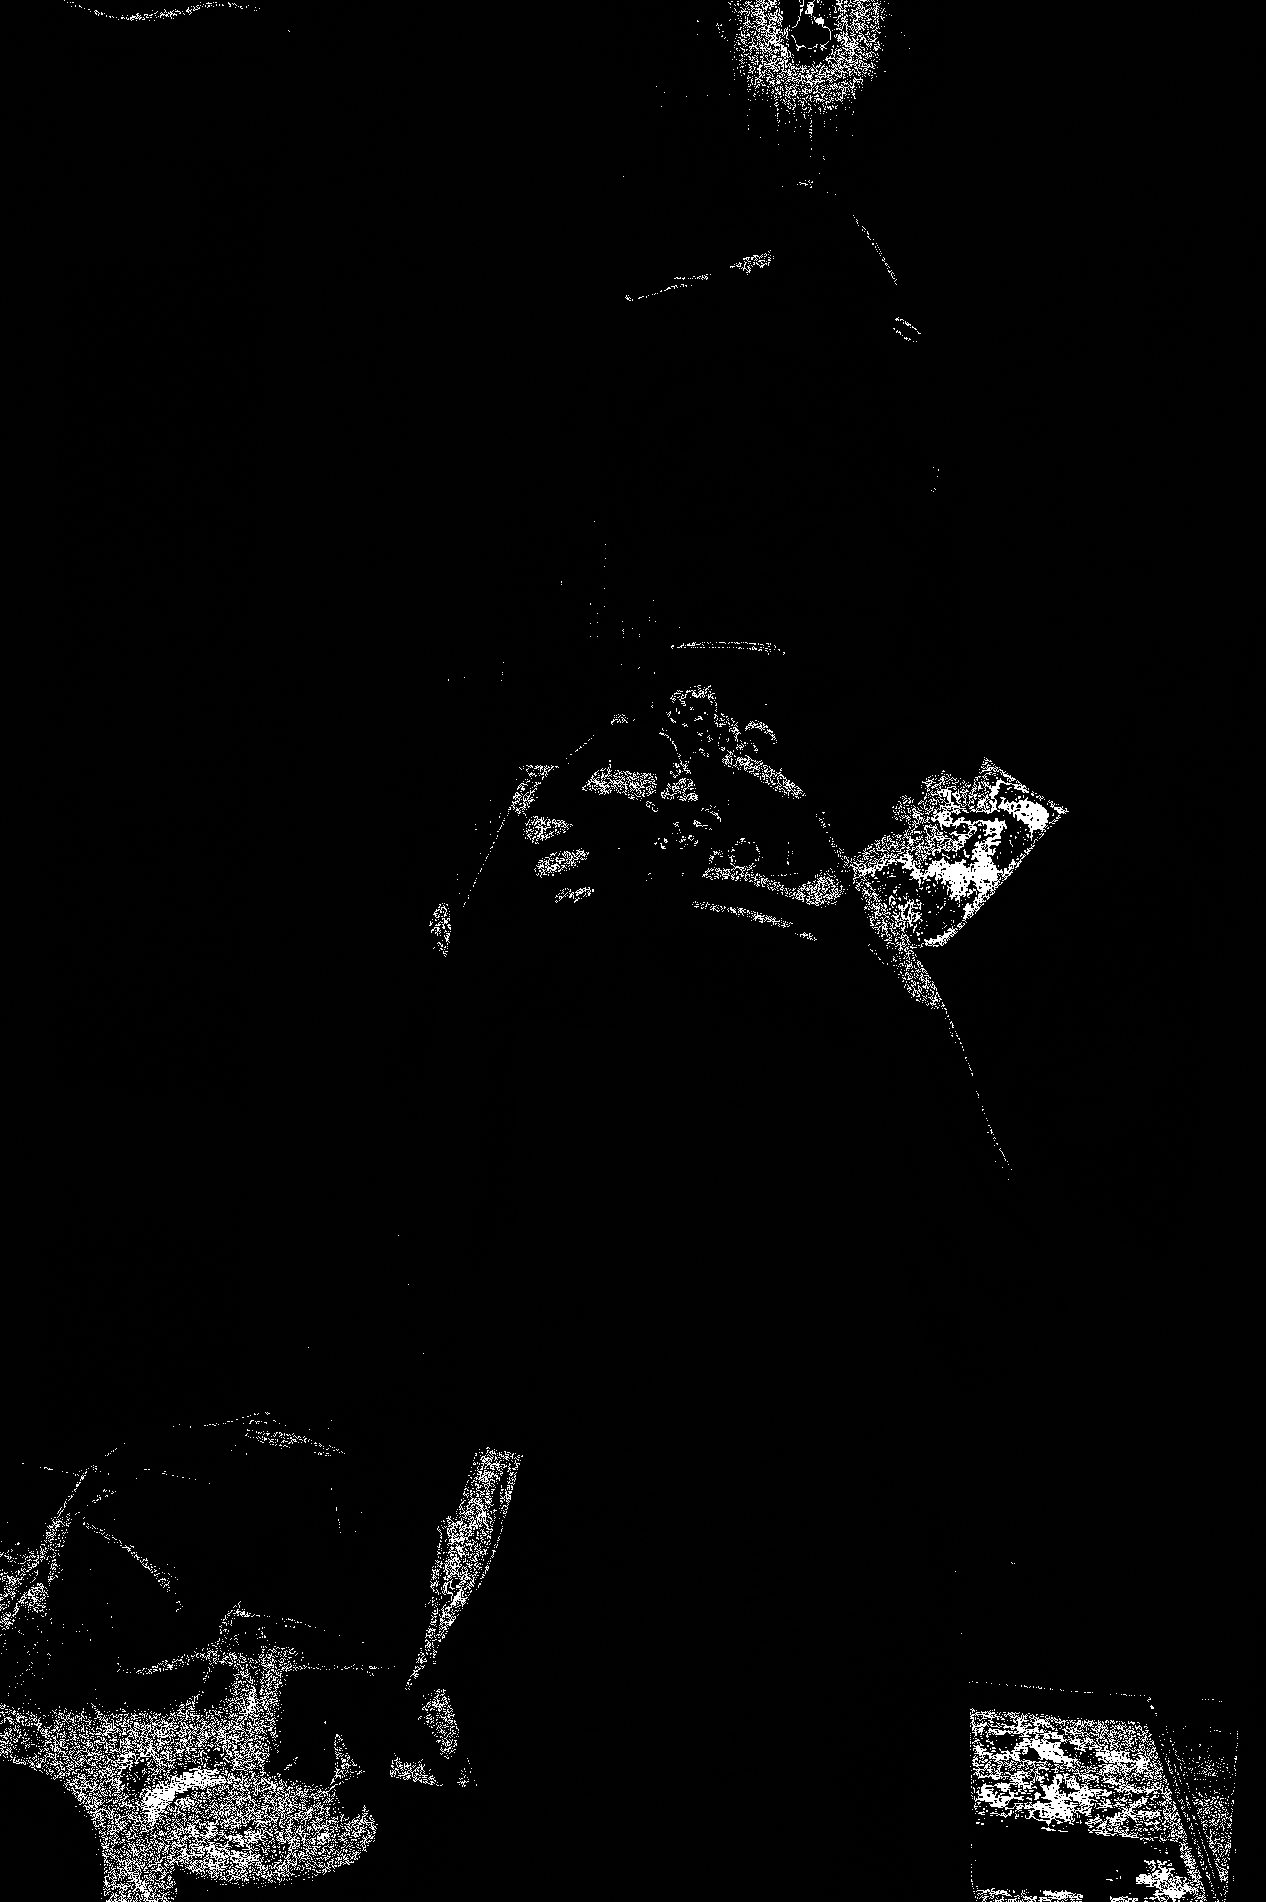
\includegraphics[width=10cm,height=7.9cm]{xuan22.png}
    \end{figure}
\end{document}